\section{Grover's algorithm}
Grover's algorithm solves unstructured search, given an unknown, oracle function and desired output $y$ it computes the value $x$ for which $f(x)=y$. \\\\
Formally we are given an oracle function:
$$f:\{0,1\}^n\rightarrow \{0,1\}$$
And we have to find an input $x\in \{0,1\}^n$ such that $f(x)=1$. \\\\
We cannot assume anything about the function properties. Therefore, without quantum search, the best approach is to guess randomly. For $M$ possible solutions to the problem, the expected number of attempts before finding a solution is ${N}/{M}$, where $N=2^n$. In contrast, Grover's algorithm can solve this task using just $\sqrt{{N}/{M}}$ function calls.
\subsection{The algorithm}
The algorithm requires $n$ qubits in the register, enough to represent all states in the function domain. We start by using $n$ Hadamard gates to set the register to the uniform state - the superposition of all states in the domain, resulting in the state $\ket{\varphi}$:
$$\ket{\varphi}=\frac{1}{M}\sum_x \ket{x}$$
Now we use the fact that all $x$ evaluate either to $0$ or $1$:
$$\forall_x: \left[x\in f^{-1}(0) \lor x\in f^{-1}(1)\right]$$
and split the sum based on that.
$$\ket{\varphi}=\frac{1}{\sqrt{N}}\left(\sum_{x\in f^{-1}(0)}\ket{x}+\sum_{x\in f^{-1}(1)}\ket{x}\right)$$ 
now we define $\ket{a}$ and $\ket{b}$ as a superposition of all possible states in $f^{-1}(0)$ and $f^{-1}(1)$ respectively: 
\begin{align*}
    \ket{a}&=\frac{1}{\sqrt{N-M}}\sum_{x \in f^{-1}(0)} \ket{x}\\
    \ket{b}&=\frac{1}{\sqrt{M}}\sum_{x \in f^{-1}(1)} \ket{x}
\end{align*}
we use $\ket{a}$ and $b$ to yet again rewrite our state:
$$\ket{\varphi}=\sqrt{\frac{N-M}{N}}\ket{a}+\sqrt{\frac{M}{N}}\ket{b}$
Using the fact that $\sqrt{\frac{N-M}{N}}^2+\sqrt{\frac{M}{N}}^2=1$ and $\sqrt{\frac{N-M}{N}}\leq 1$ and $\sqrt{\frac{M}{N}} \leq 1$ to parametrize using trigonometric function for certain angle $\theta$:
\begin{align*}
  \cos{\theta} &= \frac{N-M}{N} \\ \sin{\theta} &= \frac{M}{N}
\end{align*}
$$\ket{\varphi}=\cos{\theta} \ket{a} + \sin{\theta} \ket{b}$$
We now define a quantum gate $Q_A$ that will flip the phase of the state if $x\in f^{-1}(1)$:
$$Q_A\ket{x}=(-1)^f(x)\ket{x}$$ 
see that we can rewrite $Q_A$ as:
$$Q_A\ket{x}=\ket{a}\bra{a}\ket{x}-\ket{x}$$
we can interpret this as a reflection through the $\ket{a}$-axis, this can be easily verified, using orthogonality of $\ket{a}$ and $\ket{b}$:
\begin{align*}
  Q_A\ket{a}&=\ket{a} \\ Q_A\ket{b}&=-\ket{b}
\end{align*}
Analogously, we define an operator of reflection through $\ket{\phi}$ axis called the diffuser:
$$Q_S\ket{x}=2\ket{\varphi}\bra{\varphi}\ket{x}-\ket{x}$$
if we interpret those rotations geometrically, and assume that $M \ll N$, in the beginning we had an angle of $\ket{\theta}$ between $\ket{a}$ and $\ket{\phi}$. After we act on $\ket{\varphi}$ with $Q_S\cdot Q_A$ we get a new state $\ket{\varphi'}$, which is a rotation of $\ket{\varphi}$ by $2\theta$ towards $\ket{b}$. We attach both an illustration of this process, when plotted on the Bloch sphere on \ref{fig:grover} and Grover's algorithm quantum circuit on figure \ref{fig:grover2}
\begin{figure}[ht!]
  \begin{center}
    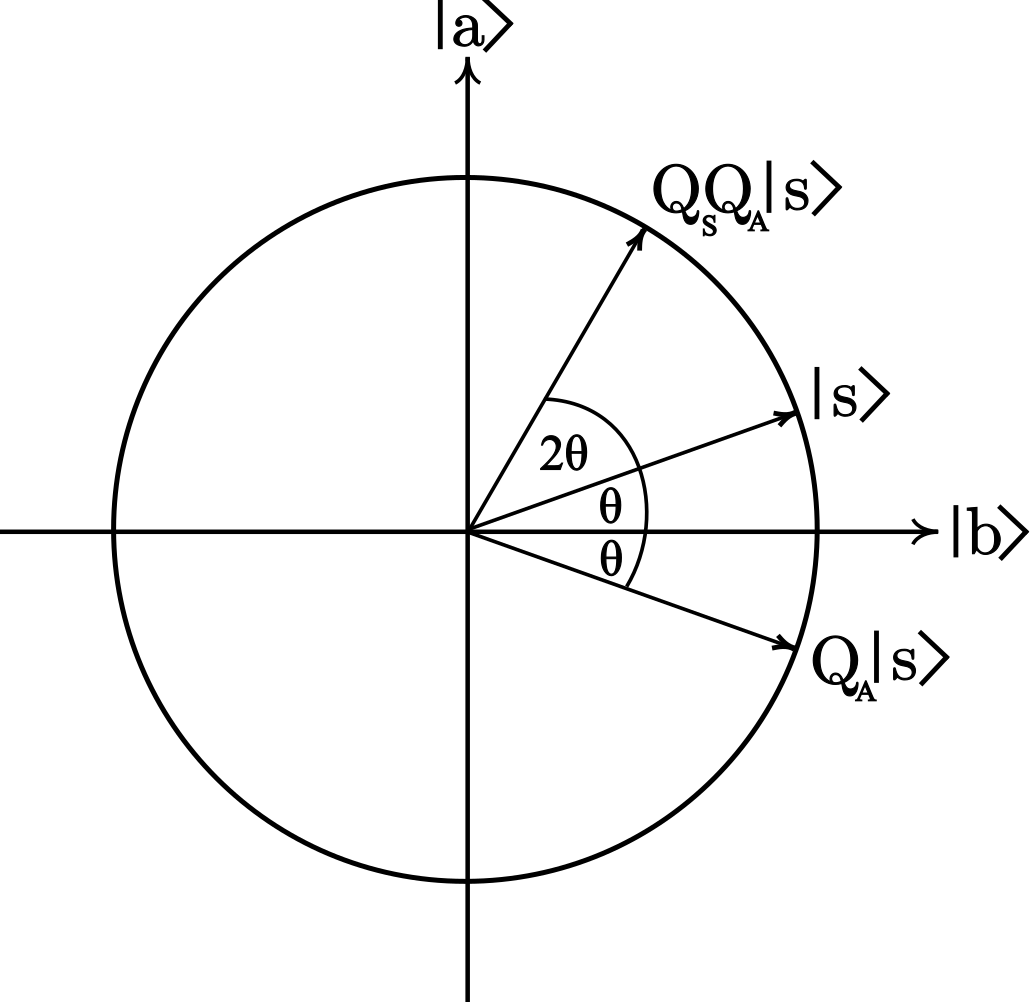
\includegraphics[width=0.5\textwidth]{figures/grover.png}
  \end{center}
  \caption{One step of Grover's search}\label{fig:grover}
\end{figure}
\begin{figure}[ht!]
  \begin{center}
    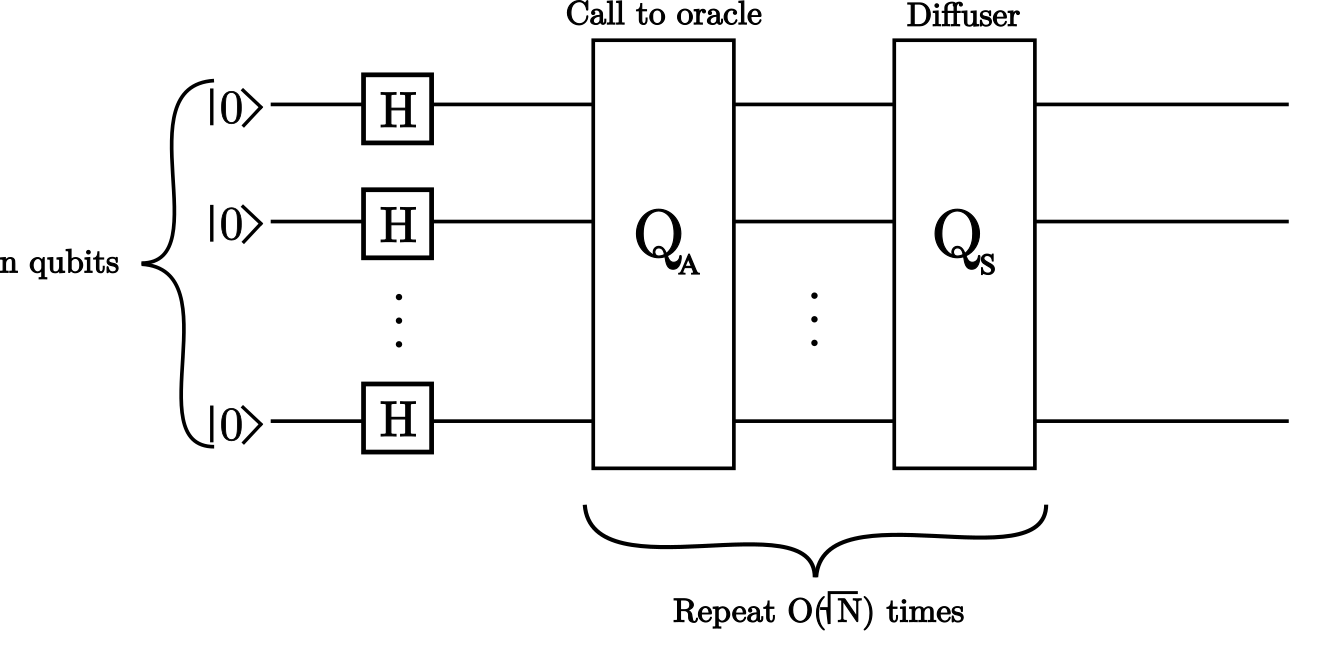
\includegraphics[width=0.9\textwidth]{figures/grover2.png}
  \end{center}
  \caption{Grover's search quantum circuit}\label{fig:grover2}
\end{figure}

\subsection{Complexity and impact}
In each step we change the angle of our state by $2 \theta$ towards $\ket{b}$ (note that $\theta$ is the same in each iteration). If we approximate $\theta$ as $\sqrt{{N}/{M}}$ we find that we need roughly $\frac{\pi}{4}\sqrt{{N}/{M}}$ steps to rotate all the way to $\ket{b}$. Then, if we measure a state close to $\ket{b}$, the probability of obtaining a valid answer is almost certain. Overall, algorithm complexity is $O(\sqrt{n})$. \\\\
Grover's algorithm solves unstructured search, an $\mathtt{NP}$-complete problem with $O(\sqrt{N})=O(\sqrt{2^n})$ steps; furthermore, we know that the algorithm is optimal - on quantum computers, there is no algorithm solving this problem with lower complexity \cite{Zalka_1999}. This means that using a quantum computer, we only get a quadratic speed-up on the problem, which makes it remain in $\mathtt{NP}$. This result led most of the experts to believe that $\mathtt{NP}$ complete problems are not possible to solve efficiently on a quantum computer.
